\documentclass[main.tex]{subfiles}
\begin{document}

\subsection{Tensor calculus}

We can define the Dalambertian operator $\square = \nabla_\mu \nabla^\mu = \nabla_\mu \partial^\mu$, which can only act on scalars, and it does so like:

\begin{equation}
    \square A = \nabla_\mu (\partial^\mu A) =  \frac{1}{\sqrt{-g}}\partial_\mu \qty(\sqrt{-g}\partial^\mu A)
\end{equation}

If we differentiate and antisymmetrize (so, take the rotor of) an antisymmetric tensor $F_{[\mu \nu]}$, the Christoffel symbols cancel:

\begin{equation}
    \nabla_{[\mu} F_{\nu\rho]} = \partial_{[\mu} F_{\nu\rho]}
\end{equation}

\paragraph{Lie derivative}

Following \cite[section 6]{Taub:1978}. The Lie derivative of a generic tensor \(T^{\mu_1 \dots \mu_n} _{\nu_1 \dots \nu_m}\) along a vector \(\xi^\mu\) is defined as:

\begin{equation}
    \Lie_{\xi} T^{\mu_1 \dots \mu_n} _{\nu_1 \dots \nu_m} \defeq
    \xi^\rho \nabla_\rho T^{\mu_1 \dots \mu_n} _{\nu_1 \dots \nu_m}
    + \sum_{i=1}^{m} T^{\mu_1 \dots \mu_n} _{\nu_1 \dots \nu_{i-1} \rho \nu_{i+1} \dots \nu_m} \nabla_{\nu_i} \xi^\rho
    - \sum_{i=1}^{n} T^{\mu_1 \dots \nu_{i-1} \rho \nu_{i+1} \dots \mu_n} _{\nu_1 \dots  \nu_m} \nabla_{\rho} \xi^{\mu_i}
\end{equation}

Some special cases are: a scalar \(\Lie _\xi f = \xi^\rho \partial_\rho f \), a vector \(\Lie _\xi u^\mu = \xi^\rho \nabla_\rho u^\mu -u^\rho \nabla_\rho \xi^\mu\), and  an antisymmetric covariant two-tensor \(\omega_{\mu\nu} = \omega_{[\mu \nu]}\) which represents a closed form \(\nabla_{[\mu} \omega_{\nu \rho]} = 0\) we have \(\Lie _\xi \omega_{\mu\nu} =2\nabla_{[\nu} \qty( \omega_{\mu] \rho} \xi^\rho )\)

\subsection{Fluid dynamics}

\paragraph{Wave velocity}

Following \cite[section 5]{Taub:1978}.

An equation in the form \(\varphi (x^\mu) = 0\) defines a 3D surface \(\Sigma\); its constant-\(x^0\) slices are 2D surfaces. We can decompose \(\partial_\mu \varphi\) in a component proportional to the velocity, \(a u_\mu\), and one which is orthogonal to it, \(W_\mu = h^\sigma_\mu \partial_\sigma \varphi\). Then \(W_\mu W^\mu = h^\sigma_\mu  h_\beta^\mu \partial_\sigma \varphi \partial^\beta \varphi = h^{\sigma\beta} \partial_\sigma \varphi \partial_\beta \varphi\)
by the idempotency of the projector \(h\).
Thus we can see that \(W^2 \geq 0\), therefore it is a spacelike vector. We can define its corresponding unit vector: \(W^\mu = t^\mu \sqrt{W^\nu W_\nu}\).

We can choose a velocity \(v\) such that \(k^\mu = u^\mu - v t^\mu\) is parallel to \(\Sigma\), or \(k^\mu \partial_\mu \varphi = 0\). If this condition is satisfied, then \(v\) is the wave velocity of \(\Sigma\) as measured by an observer with velocity \(u^\mu\).

\begin{figure}[ht]
  \centering
  \incfig{figures/taub_wave_velocity}
  \caption{Wave velocity diagram}
  \label{fig:taub_wave_velocity}
\end{figure}

Now, we can multiply the equation \(k^\mu = u^\mu - v t^\mu\) by \(\partial_\mu \varphi\): we get \(v t^\mu \partial_\mu \varphi = u^\mu \partial_\mu \varphi\). What multiplies \(v\) in the LHS of this equation is the length of the spatial component of \(\partial_\mu \varphi\), or \(\sqrt{h^{\mu\nu} \partial_\mu \varphi \partial_\nu \varphi}\).
Using the definition of \(h ^{\mu \nu} \), we can arrive at

\begin{equation} \label{eq:lorentz-factor-wave-velocity}
    \gamma^{-2} = 1 - v^2 = \frac{g^{\mu\nu} \partial_\mu \varphi \partial_\nu \varphi}{h^{\mu\nu} \partial_\mu \varphi \partial_\nu \varphi}
\end{equation}

The denominator in \eqref{eq:lorentz-factor-wave-velocity} is positive, so we can see that \(1-v^2\) is positive iff \(\partial_\mu \varphi\) is spacelike, and \(v^2 = 1\) iff it is null.

If we are dealing with a timelike surface \(\Sigma\), or equivalently \(\partial_\mu \varphi\) is spacelike, then we define \(n^\mu \propto \partial_\mu \varphi\) such that \(n^\mu n_\mu = 1\) and we find:

\begin{equation}
    v = \frac{u^\mu \partial_\mu \varphi}{\sqrt{h^{\mu\nu} \partial_\mu \varphi \partial_\nu \varphi}}
    = \frac{u^\mu n_\mu}{\sqrt{h^{\mu\nu} n_\nu n_\mu}}
    = \frac{u^\mu n_\mu}{\sqrt{1 + (u^\mu n_\mu)^2}}
\end{equation}

From this it can be shown that \(1-v^2 = (1+(u^\mu n_\mu)^2)^{-1}\), and then \(v \gamma = u^\mu n_\mu\).

\paragraph{Stationarity}

Will skip most of this section. A spacetime is stationary if it admits a timelike Killing vector field? \textcite[]{Ehlers:1971} proved that from a hypothesis of stationarity we get \(\nabla_\mu S^\mu = 0\).

\paragraph{Speed of sound}

Following \cite[]{Yoshida:2011}.
We want to justify the expression \(v_s^2 = \pdv*{p}{\rho} \). We work in Minkowski spacetime, where \(g_{\mu\nu} = \eta_{\mu\nu}\), and with an ideal fluid, for which \(T_{\mu\nu} = (p+ \rho) u_\mu u_\nu + p \eta_{\mu\nu}\). Then, the equations of conservation of mass and momentum read:

\begin{subequations}
\begin{align}
  \rho_0 \partial_\mu u^\mu + u^\mu \partial_\mu \rho_0 &= 0 & \text{mass}  \\
  u^\mu \qty(\partial_\mu \rho - h \partial_\mu \rho_0) &=0 & \text{momentum along } u^\mu  \\
  (p+\rho) a^\mu + h^{\mu \rho} \partial_\rho p &=0 & \text{momentum in the span of } h_{\mu\nu}
\end{align}
\end{subequations}

where \(h\) is the specific enthalpy. If we assume small perturbations \(p \rightarrow p + \delta p\), \(\rho_0 \rightarrow \rho_0 + \delta \rho_0\), \(\rho \rightarrow \rho + \partial \rho\), \(u^\mu \rightarrow (1, \delta u^x, 0, 0)\) (it is \emph{almost} normalized) we get our three equations, up to first order in the perturbations:

\begin{subequations}
\begin{align}
  \partial_x (\delta u^x) &= -\frac{\partial_t (\delta \rho_0)}{\rho_0}  \\
  \partial_t (\delta \rho) - h \partial_t (\delta \rho_0) &= 0  \\
  -(p+ \rho) \partial_t (\delta u^x) &= \partial_x p
\end{align}
\end{subequations}

We manipulate these by differentiating and substituting, in order to eliminate the dependence on \(\delta u^x\) and \(\rho_0\), and get:

\begin{subequations}
\begin{align}
  \partial_t \delta \rho + (p+\rho) \partial_x (\partial u^x) &= 0 \\
  \partial_x \delta p + (p+\rho) \partial_t (\partial u^x) &= 0
\end{align}
\end{subequations}

which simplifies to \(\partial_{tt}^2 \delta \rho - \partial_{xx}^2 \delta p = 0\): in order to get the wave equation in the form \(\qty(v_s^{-2} \partial_{tt}^2 - \partial_{xx}^2 ) \delta p = 0\) we \emph{need} to define \(v_s^2 = \pdv*{p}{\rho}\).

\paragraph{Barotropic flows}

The definition of a barotropic flow is: a flow for which the density is just a function of temperature, \(\rho = \rho (p)\).

\begin{greenbox}
  What is \(d\) in \cite[equation 11.10]{Taub:1978}? Is it a typo? I do not get that equation. Also, I quote: ``Equations 11.3 and 11.5 do not hold. However, it is a consequence of equations 11.3 and...''.

  Insert here: definition of the variable \(s\).
\end{greenbox}

The quantity \(s\) obeys the conservation law \(\nabla_\mu (s u^\mu) = 0\). We define a quantity \(Q = \log ((\rho + p)/s )\), which for \(s=\rho_0\) is the log-enthalpy. Then, the Euler equation \eqref{eq:relativistic-euler} can be substituted by

\begin{equation}
  a^\sigma = - h^{\sigma \mu} \partial_\mu Q
\end{equation}

or, more explicitly:

\begin{equation}
  (\rho + p) a^\mu = -s h^{\mu\nu} \partial_\nu \qty(\frac{\rho + p}{s})
\end{equation}

\begin{greenbox}
  Unproven in \cite[]{Taub:1978}!? where does it come from?
\end{greenbox}

We now define a ``current'' of \(\exp(Q)\): \(V^\mu = \exp(Q) u_\mu \).

Then we define \(\Omega_{\mu\nu} = 2 \nabla_{(\mu} V_{\nu)}\): this satisfies \(\Omega_{\mu\nu} u^\nu = - T \partial_\mu S\) in general, and \(\Omega_{\mu\nu} u^\nu = 0\) in the isentropic case.

\begin{greenbox}
  Right? Underneath equation \cite[11.14]{Taub:1978} what is meant is ``in the isentropic'' case, I think, since then \(\partial_\mu S = 0\)...

  Also, what does the distinction between the two definitions in 11.14 and 11.13 mean? Is 11.13 not a subcase of 11.14?
\end{greenbox}

Then, we define

\begin{equation}
  v^\mu = \frac{1}{2} \eta^{\mu \nu \rho \sigma} u_\nu \Omega_{\rho \sigma}
\end{equation}

which satisfies

\begin{equation}
  3 u_{[\alpha} \Omega_{\beta \gamma]} = v^{\mu} \eta_{\mu \alpha \beta \gamma}
\end{equation}

\begin{greenbox}
  The normalization does not seem right: \(\eta^{\mu\nu\rho\sigma} \eta_{\mu\alpha\beta\gamma} = -\delta^{\nu\rho\sigma}_{\alpha\beta\gamma}\), so when substituting in the result seems off by \(- 3!\)...
\end{greenbox}

We use this result to get an explicit formula for \(\Omega_{\alpha\beta}\) in terms of \(u^\mu\), \(v^\mu\).
This comes out by multiplying by \(u^\gamma\), and is:

\begin{equation}
  \Omega _{\alpha\beta}
  = - v^\mu u^\gamma \eta_{\mu\gamma\alpha\beta} + u_\alpha \Omega_{\beta\gamma} u^\gamma - u_\beta \Omega_{\alpha\gamma} u^\gamma
  = - v^\mu u^\gamma \eta_{\mu\gamma\alpha\beta} + 2T (u_{[\beta} \partial_{\alpha]} S )
\end{equation}

We can also rewrite the perfect-fluid stress-energy tensor as \(T^{\mu\nu} = s V^\mu u^\nu +p g^{\mu\nu}\): then, since the metric has zero covariant derivative, if we look at the projection of \(T^{\mu\nu}\) along a Killing vector field \(\nabla_{(\mu} \xi_{\nu)}=0\) we get

\begin{equation}
  \nabla_\nu \qty(\xi_\mu T^{\mu\nu}) = \nabla_\nu \qty(\xi_\mu s V^\mu u^\nu) = 0
\end{equation}

but in the (barotropic?) case \(s = \rho_0\) we can use the conservation of mass to get \(\rho_0 u^\nu \nabla_\nu (\xi_\mu V^\mu) = 0\), so the quantity \(H = \xi_\mu V^\mu\) is conserved along the worldlines of the fluid.

If we are in the coordinate system which would be the LRF for an observer with velocity \(\xi^\mu\), then the conserved quantity is \(H = V^0 \).

\paragraph{Shocks and conservation laws through boundaries}

Following \cite[section 13]{Taub:1978}.
The differential formulations of the conservation of mass and momentum will not hold at points of non-differentiability, such as through shock waves.
There, they must be replaced by an integral law.
We can reframe our conservation laws as the statements that, for any scalar \(f\) and vector \(\lambda_\mu\) we will have

\begin{subequations} \label{eq:conservation-laws-arbitrary-functions}
\begin{align}
  \nabla_\mu \qty(f \rho_0 u^\mu) &= \rho_0 u^\mu \partial_\mu f  \\
  \nabla_\mu \qty(\lambda_\nu T^{\mu\nu})&= T^{\mu\nu} \nabla_\mu \lambda_\nu
\end{align}
\end{subequations}

We can integrate these on a generic volume \(V\) using Stokes' theorem \eqref{eq:stokes-theorem}, choosing coordinates on the boundary such that the determinant of the induced metric on the submanifold is uniformly 1.

\begin{subequations} \label{eq:conservation-laws-arbitrary-functions-integral}
    \begin{align}
        \int _{\partial V} n_\mu \qty(f \rho_0 u^\mu) \dd[3]{y} &= \int_V \rho_0 u^\mu \partial_\mu f \sqrt{-g}  \dd[4]{x}  \\
        \int_{\partial V} n_\mu \qty(\lambda_\nu T^{\mu\nu}) \dd[3]{y}&= \int _V T^{\mu\nu} \nabla_\mu \lambda_\nu \sqrt{-g}  \dd[4]{x}
    \end{align}
\end{subequations}

Now, to deal with the shock we do the following: take the hypersurface at which the shock happens, enclose it in an infinitesimally thin 4D volume: then, as the volume decreases the RHSs of equations \eqref{eq:conservation-laws-arbitrary-functions-integral} go to 0, therefore the LHSs also must: we can write them as the difference of the integrands at the boundary.
Therefore, introducing the notation \([F] = F_+ - F_-\), selecting one of the two outward vectors and denoting only it as \(n_\mu\) and using the arbitrariness of \(f\), \(\lambda_\nu\) we have:

\begin{equation}
    \qty[n_\mu \rho_0 u^\mu] = n_\mu \qty[\rho_0 u^\mu] = 0
    \qquad
    \text{and}
    \qquad
    \qty[n_\mu T^{\mu\nu}] = n_\mu [T^{\mu\nu}] = 0
\end{equation}

We denote \(m = \rho_0 u^\mu n_\mu\) (at the boundary), and then the first equation is the fact that \(m\) is the same on either side:

\begin{equation} \label{eq:rankine-hugoniot-1}
    \rho_{0+} u^\mu_+ n_\mu =
    \rho_{0-} u^\mu_- n_\mu \defeq m
\end{equation}

The other, for an ideal flud, is

\begin{equation} \label{eq:momentum-conservation-across-boundary}
    m \qty(V^\mu_+ - V^\mu _-) + n^\mu \qty(p_+ - p_-) = 0
\end{equation}

with \(V^\mu = h u^\mu\). Now, consider a set of vectors \(Y^\mu\) such that \(Y^\mu n_\mu = 0\) and \(Y^\mu Y_\mu = 1\). These form a two-parameter family (\(\sim S^2\)), and
by \eqref{eq:momentum-conservation-across-boundary} must satisfy

\begin{equation}
    m \qty(V^\mu_+ - V^\mu _-) Y_\mu = 0
\end{equation}

then
\begin{itemize}
    \item either \(m = 0\): this is called a \emph{slip-stream} discontinuity, because the normal component of the velocity is zero, so the fluid is flowing \emph{along} the boundary, no matter is crossing it;
    \item  or \(V^\mu _+ Y_\mu = V^\mu _- Y_\mu\) for \emph{all} the \(Y^\mu\): this is called a \emph{shock wave}.
\end{itemize}

\begin{greenbox}
  There are \emph{three} independent \(Y^\mu\), right?
\end{greenbox}

In the shock wave case, we must write two (?) more equations to fully recover the \eqref{eq:momentum-conservation-across-boundary}. To do so, we define \(\tau = h/\rho_0\) and use the fact that \(V^2 = -h^2\).
Then, we multiply \eqref{eq:momentum-conservation-across-boundary} by \(V_{\mu}^{+}\) and \(V_{\mu}^{-}\), and use the fact that \(n_\mu V^\mu_{\pm} = m \tau_{\pm}\). We get

\begin{equation} \label{eq:rankine-hugoniot-2}
    h^2_+ - h^2_- - (p_+ - p_-)(\tau_+ - \tau_-) = 0
\end{equation}

then, by multiplying \eqref{eq:momentum-conservation-across-boundary} and using the fact that \(n^\mu\) is timelike we get:

\begin{equation}\label{eq:rankine-hugoniot-3}
    m^2 = \frac{p_+ - p_-}{\tau_+ - \tau_-}
\end{equation}

equations \eqref{eq:rankine-hugoniot-1}, \eqref{eq:rankine-hugoniot-2} and \eqref{eq:rankine-hugoniot-3} are the Rankine-Hugoniot equations.

\begin{greenbox}
  TODO: show that the nonrelativistic limit of these is

  \begin{subequations}
  \begin{align}
    \rho_0 u^i n_i &= \const  \\
    \rho_0 u^i u_i + p &= \const  \\
    h + u^2 /2 &= \const
  \end{align}
  \end{subequations}
\end{greenbox}

\subsection{Radiative processes}

\begin{greenbox}
  Question posed in \cite[Introduction]{ThorneFLammmangZytkow:1981feb}: will a black hole inside a star eat it whole in a free-fall time-scale (around 1 year) or on an Eddington-limited time-scale (around \(10^8\) years)?
  Is this known now?
\end{greenbox}

\paragraph{Eddington luminosity}

It is the characteristic luminosity at which the radiation pressure from the photons moving outward equals the gravitational specific force on the infalling matter.

The gravitational force, in the newtonian  limit, is

\begin{equation}
  F_{\text{grav}} = \frac{GMm}{r^2 }
\end{equation}

The radiation pressure can be given in terms of the luminosity \(L\) (reinserting the units of \(c\) for this) as

\begin{equation}
  P_{\text{rad}} = \frac{L}{c 4 \pi r^2}
\end{equation}

then, the radiative force is given by \(F_{\text{rad}} =  P_{\text{rad}} \kappa m\), where \(m\) is the mass of the test object and \(\kappa\) is the opacity: the per-unit-mass cross-section. We usually assume \(\kappa = \sigma_T/m_p\), that is, that the interaction between radiation and matter is all due to Thompson scattering and the matter is only composed of hydrogen atoms.

Equating the forces, we get our result:

\begin{equation}
 \frac{L_{\text{Edd}}}{M} = \frac{4 \pi c G}{\kappa}
\end{equation}

In the \(\kappa = \sigma_T / m_p \approx \SI{0.04}{\metre^2 / kg}\) case, we get \(L_{\text{Edd}} / M\) to be around \SI{6.32}{\watt\per\kilo\gram} (constants' values from \cite[]{NISTReccomendedConstants:2018}).
If we express this in units of \(L_{\odot} / M_{\odot} \approx \SI{1.93E-04}{\watt\per\kilo\gram}\) \cite[]{SunFactSheet:2018} we get \(L_{\text{Edd}} / M \approx  \num{3.27E+04} L_{\odot} / M_{\odot}\):
the amount of radiation emitted by the Sun is much less than the Eddington limit.

It is, of course, important to note that this is a limit found with many approximations: nonrelativistic gravity, spherical symmetry, only Thompson scattering, only hydrogen.

\paragraph{Cooling function}

From \cite{NobiliTurollaZampieri:1991dec}.

The cooling function \(\Lambda (T)\) is defined by the following relation, which describes the variation in the energy density by radiative processes:

\begin{equation}
    \dv{U}{t} = n^2_b \qty(\Gamma(T) - \Lambda (T))
\end{equation}

where \(U\) is the energy density (measured in \si{\erg\per\cubic\centi\metre}), \(n_b\) is the baryon density (measured in \si{\per\cubic\centi\metre}), while \(\Gamma\) and \(\Lambda\) are the heating and cooling functions, both measured in \si{\erg\cubic\centi\metre\per\second}, see \cite[equation 1]{GnedinHollon:2012}.

The cooling function of the infalling gas is

\begin{figure}
    \centering
    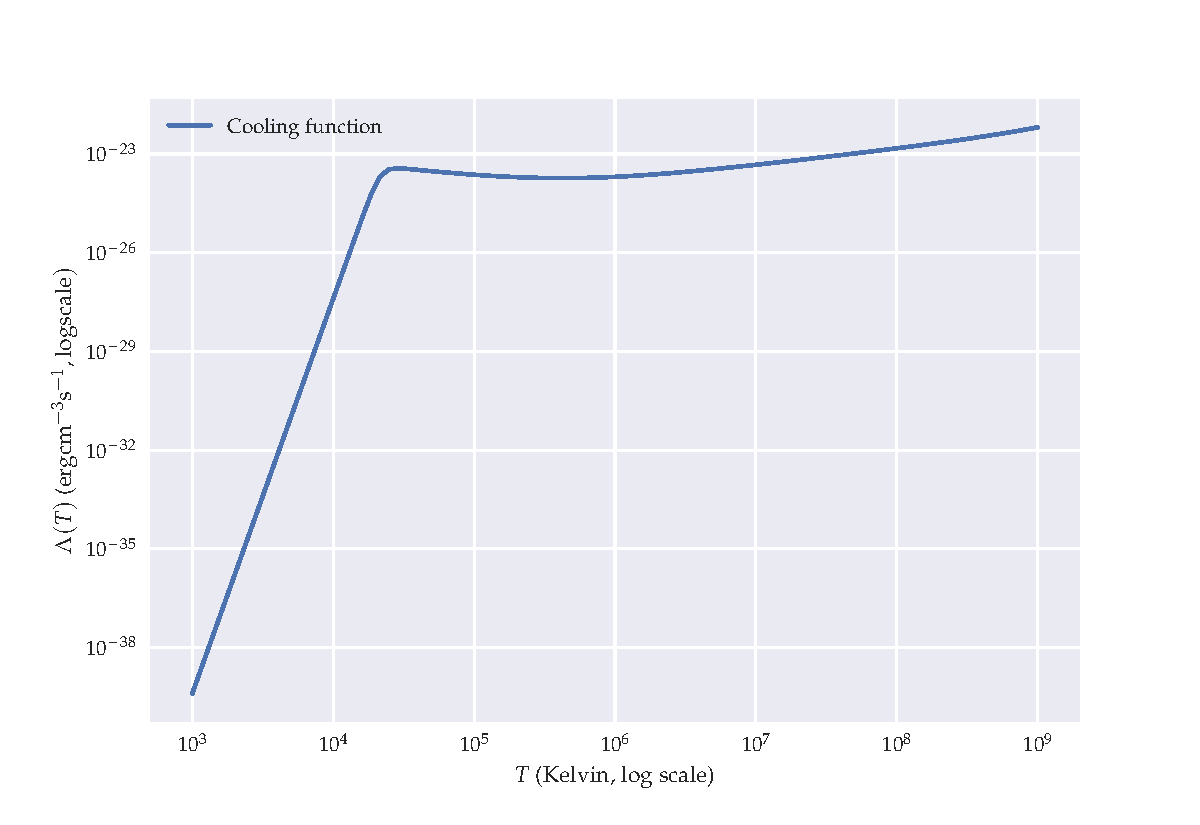
\includegraphics[width=\textwidth]{figures/cooling_function.pdf}
    \caption{Cooling function graph.}
    \label{fig:cooling-function}
\end{figure}

\begin{equation} \label{eq:cooling-function-NTZ91} 
    \begin{split}
    \Lambda (T) &= \left(
    \qty(
    \num{1.42e-27}T^{1/2} \qty(
    1 + \num{4.4e-10}T
    ) + \num{6.0e-22}T^{-1/2}
    )^{-1} \right. \\
    & \quad \left. + \num{e25} \qty(\frac{T}{\SI{1.5849e4}{K}})^{-12}
    \right)^{-1} \si{\erg\cubic\centi\metre\per\second}
    \end{split}
\end{equation}

The version of this equation in \textcite[equation 10]{StellingwerfBuff:1982} is similar: the first constant is \(\SI{2.4e-27}{} \) instead of \(\SI{1.42e-27}{} \), and the factor \(\qty(1 + \SI{4.4e-10}{}T)\) is just \(1\).


\end{document}
